\documentclass{article}

\usepackage{graphicx} % for images
\usepackage{amsmath} % for math
\usepackage{amssymb} % for \mathbb
\usepackage{siunitx} % for \SI, \num
\usepackage{hyperref} % for \url{}

% This stuff is for figures
\usepackage{float}
\DeclareGraphicsExtensions{.pdf, .png, .jpg}

% coloring of links for PDF format
\hypersetup{
    colorlinks=true,
    urlcolor=blue,
    linkcolor=black
}

% \c command redefinition (for monospaced font)
\renewcommand{\c}[1]{\texttt{#1}}
% \today command re-definition
%https://tex.stackexchange.com/questions/112932/today-month-as-text
\renewcommand{\today}{\ifnum\number\day<10 0\fi \number\day \space%
\ifcase \month \or January\or February\or March\or April\or May%
\or June\or July\or August\or September\or October\or November\or December\fi\space%
\number \year} 

\begin{document}
\begin{titlepage}
	\centering
	
\includegraphics[width=0.25\textwidth]{Images/247px-CSU-Longbeach_seal}\par\vspace{1cm}
	{\scshape\Large California State University, Long Beach \par}
	\vspace{1cm}
	{\scshape\Large CECS 447\par}
	\vspace{1.5cm}
	{\huge\bfseries Project 2\par}
	\vspace{2cm}
    {\Large\itshape Rodrigo Becerril Ferreyra\par}
    {\itshape\Large Student ID 017584071 \par}
	\vfill
    A project that demonstrates the ARM Cortex-M4
	microcontroller's UART serial capabilities.

	\vfill

% Bottom of the page
	{\large \today\par}
\end{titlepage}

\section{Introduction}
This project tasks us students to create a system that utilizes
Universal Asynchronous Receiver-Transmitter (UART) serial
communication for different purposes. The project uses two
MCUs named MCU1 and MCU2. Depending on the mode,
the system can use only one MCU, can be in a symmetrical
configuration, or can be in a master/slave configuration.
MCU1 is connected to a serial port
on a personal computer, while MCU2 is connected to MCU1 by two
cables (i.e. it is not connected to the PC). There are three
modes that this system works under:
\begin{enumerate}
	\item Mode 1 ignores the slave MCU and only utilizes the 
	MCU1. The MCU displays a prompt on the screen.
	The user can then type in a single character---either \c{r},
	\c{g}, \c{b}, \c{p}, \c{w}, or \c{d}---in order to
	change the color of the on-board LED to red, green, blue,
	purple, white, or dark (off), respectively.
	\item Mode 2 uses both MCUs in a symmetrical configuration.
	Pressing the left on-board button on any board cycles the
	LED of that board to another color. Pressing the right
	on-board button sends the color to the other MCU, which
	changes them to the same color. The color change and sending
	can be initiated by any MCU.
	\item Mode 3 has the MCUs in a master/slave configuration.
	First, the user is prompted to input a string of text on
	his or her PC. The text is sent to the master, which is
	relayed to and processed by the slave.
	The slave then sends back a modified
	version of the input, and the master again relays the
	modified string to the PC for the user to view.
\end{enumerate}

The user can change modes by clicking an external button, which
kicks the user into a menu to select the mode.

\section{Operation}
I wrote only one program for this project, but the two MCUs can
run different code depending on the mode. In order to
achieve this, Line 27 of \c{main.c} allows the user to choose
to program either MCU1 or MCU2. To program MCU1, the user must
set the \c{masterorslave} \c{enum} to the value \c{MASTER}.
This selects code that only the master MCU runs. The program
then must be compiled and flashed onto MCU1. (Make sure that
there is only one LaunchPad connected to the computer while
flashing.) To program MCU2,
set \c{masterorslave} to \c{SLAVE}, compile the program, and
flash it onto MCU2.

Here's a link to a video displaying how the system works:
\url{https://youtu.be/gnqW8FKfQK8}

\section{Theory}
When the two MCUs are communicating with each other,
in order to ensure that the receiving MCU obtains the correct
data from the transmitting MCU, both MCUs must go through a
``handshake process'' that verifies that the correct data
has been sent and receive. The handshake process is listed below.
In this model, ``data'' is defined as a single byte that is
transmitted that represents a printable character, ``\c{ENQ}''
is the ASCII enquiry bit (value \c{0x5}), and ``\c{ACK}'' is
the ASCII acknowledge bit (value \c{0x6}).
\begin{enumerate}
	\item The transmitter sends the data to the receiver. The
	receiver then saves the data.
	\item The transmitter sends \c{ENQ}, to ask if it is OK
	to send the next datum.
	\item The receiver sends \c{ACK}, saying that it is ready
	to receive the datum.
	\item If there is more data to send, jump to Step 1. If
	there is no more data to send, then exit.
\end{enumerate}

This system is used every single time there is
\emph{more than one
byte of data} to send. This is used throughout Mode 3, and
during the mode-change interrupt (where MCU2 alerts MCU1
that it is ready to receive the new mode value from MCU1).
The only time board-to-board communication is implemented not
using this protocol is during Mode 2, since only one byte of
data is transmitted.

I had much trouble figuring this handshake algorithm out,
but now that it is implemented, I get a high accuracy in my
sends and receives.

\section{Hardware Design}
I put \SI{10}{\kilo\ohm} resistors between the \c{UART1} serial
ports (\c{B0} and \c{B1}) just in case failing to do so would
fry either board. This is because, if one pin is at
\SI{3.3}{\volt} and another pin is at \SI{0}{\volt}
with no resistance betweeen them, that means
that there might be infinite current between the two pins.
I did not want to take that chance.

\begin{figure}[H]
	\centering
	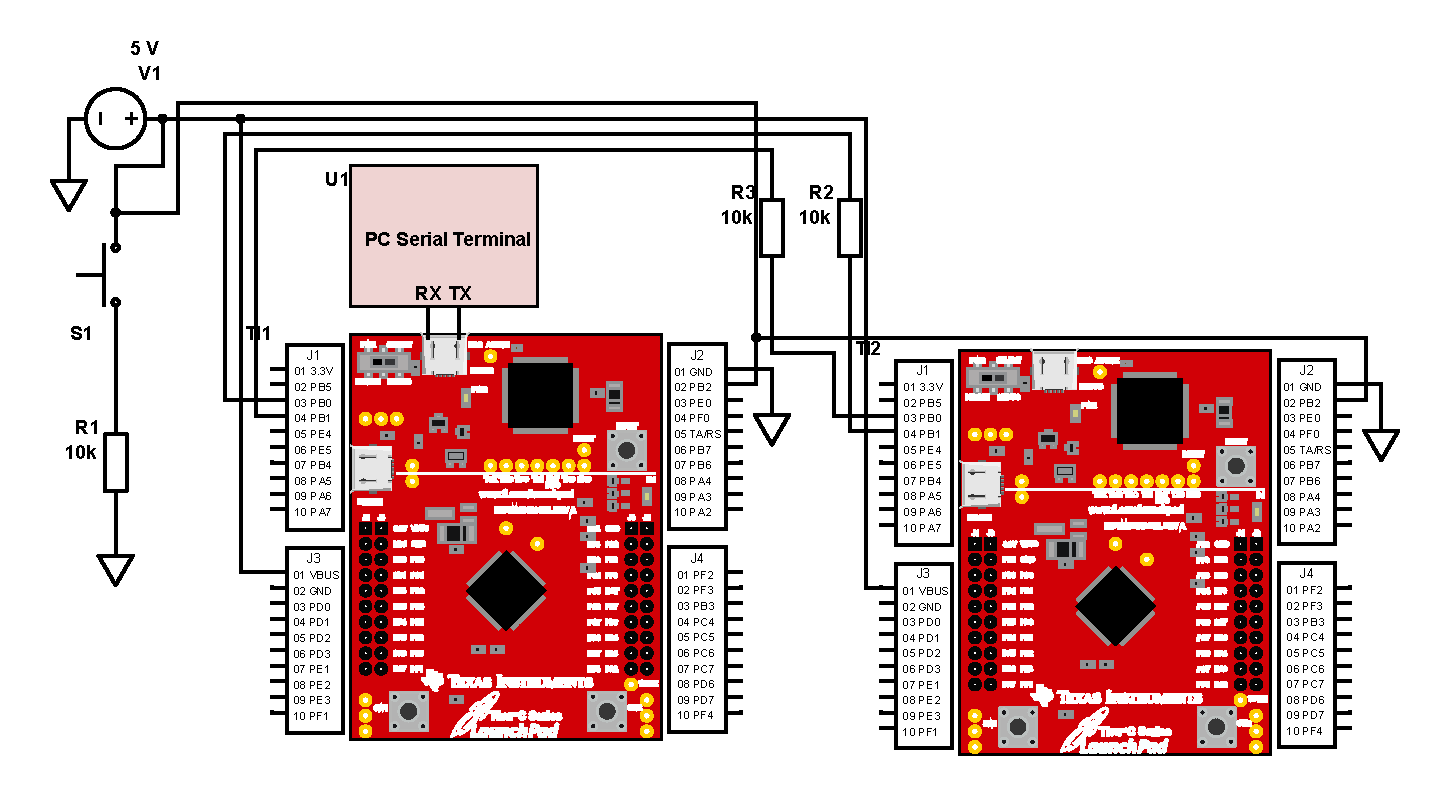
\includegraphics[width=\textwidth]{Images/schematic-diagram}
	\caption{The schematic diagram of the embedded system.}
	\label{diagram}
\end{figure}

\begin{figure}[H]
	\centering
	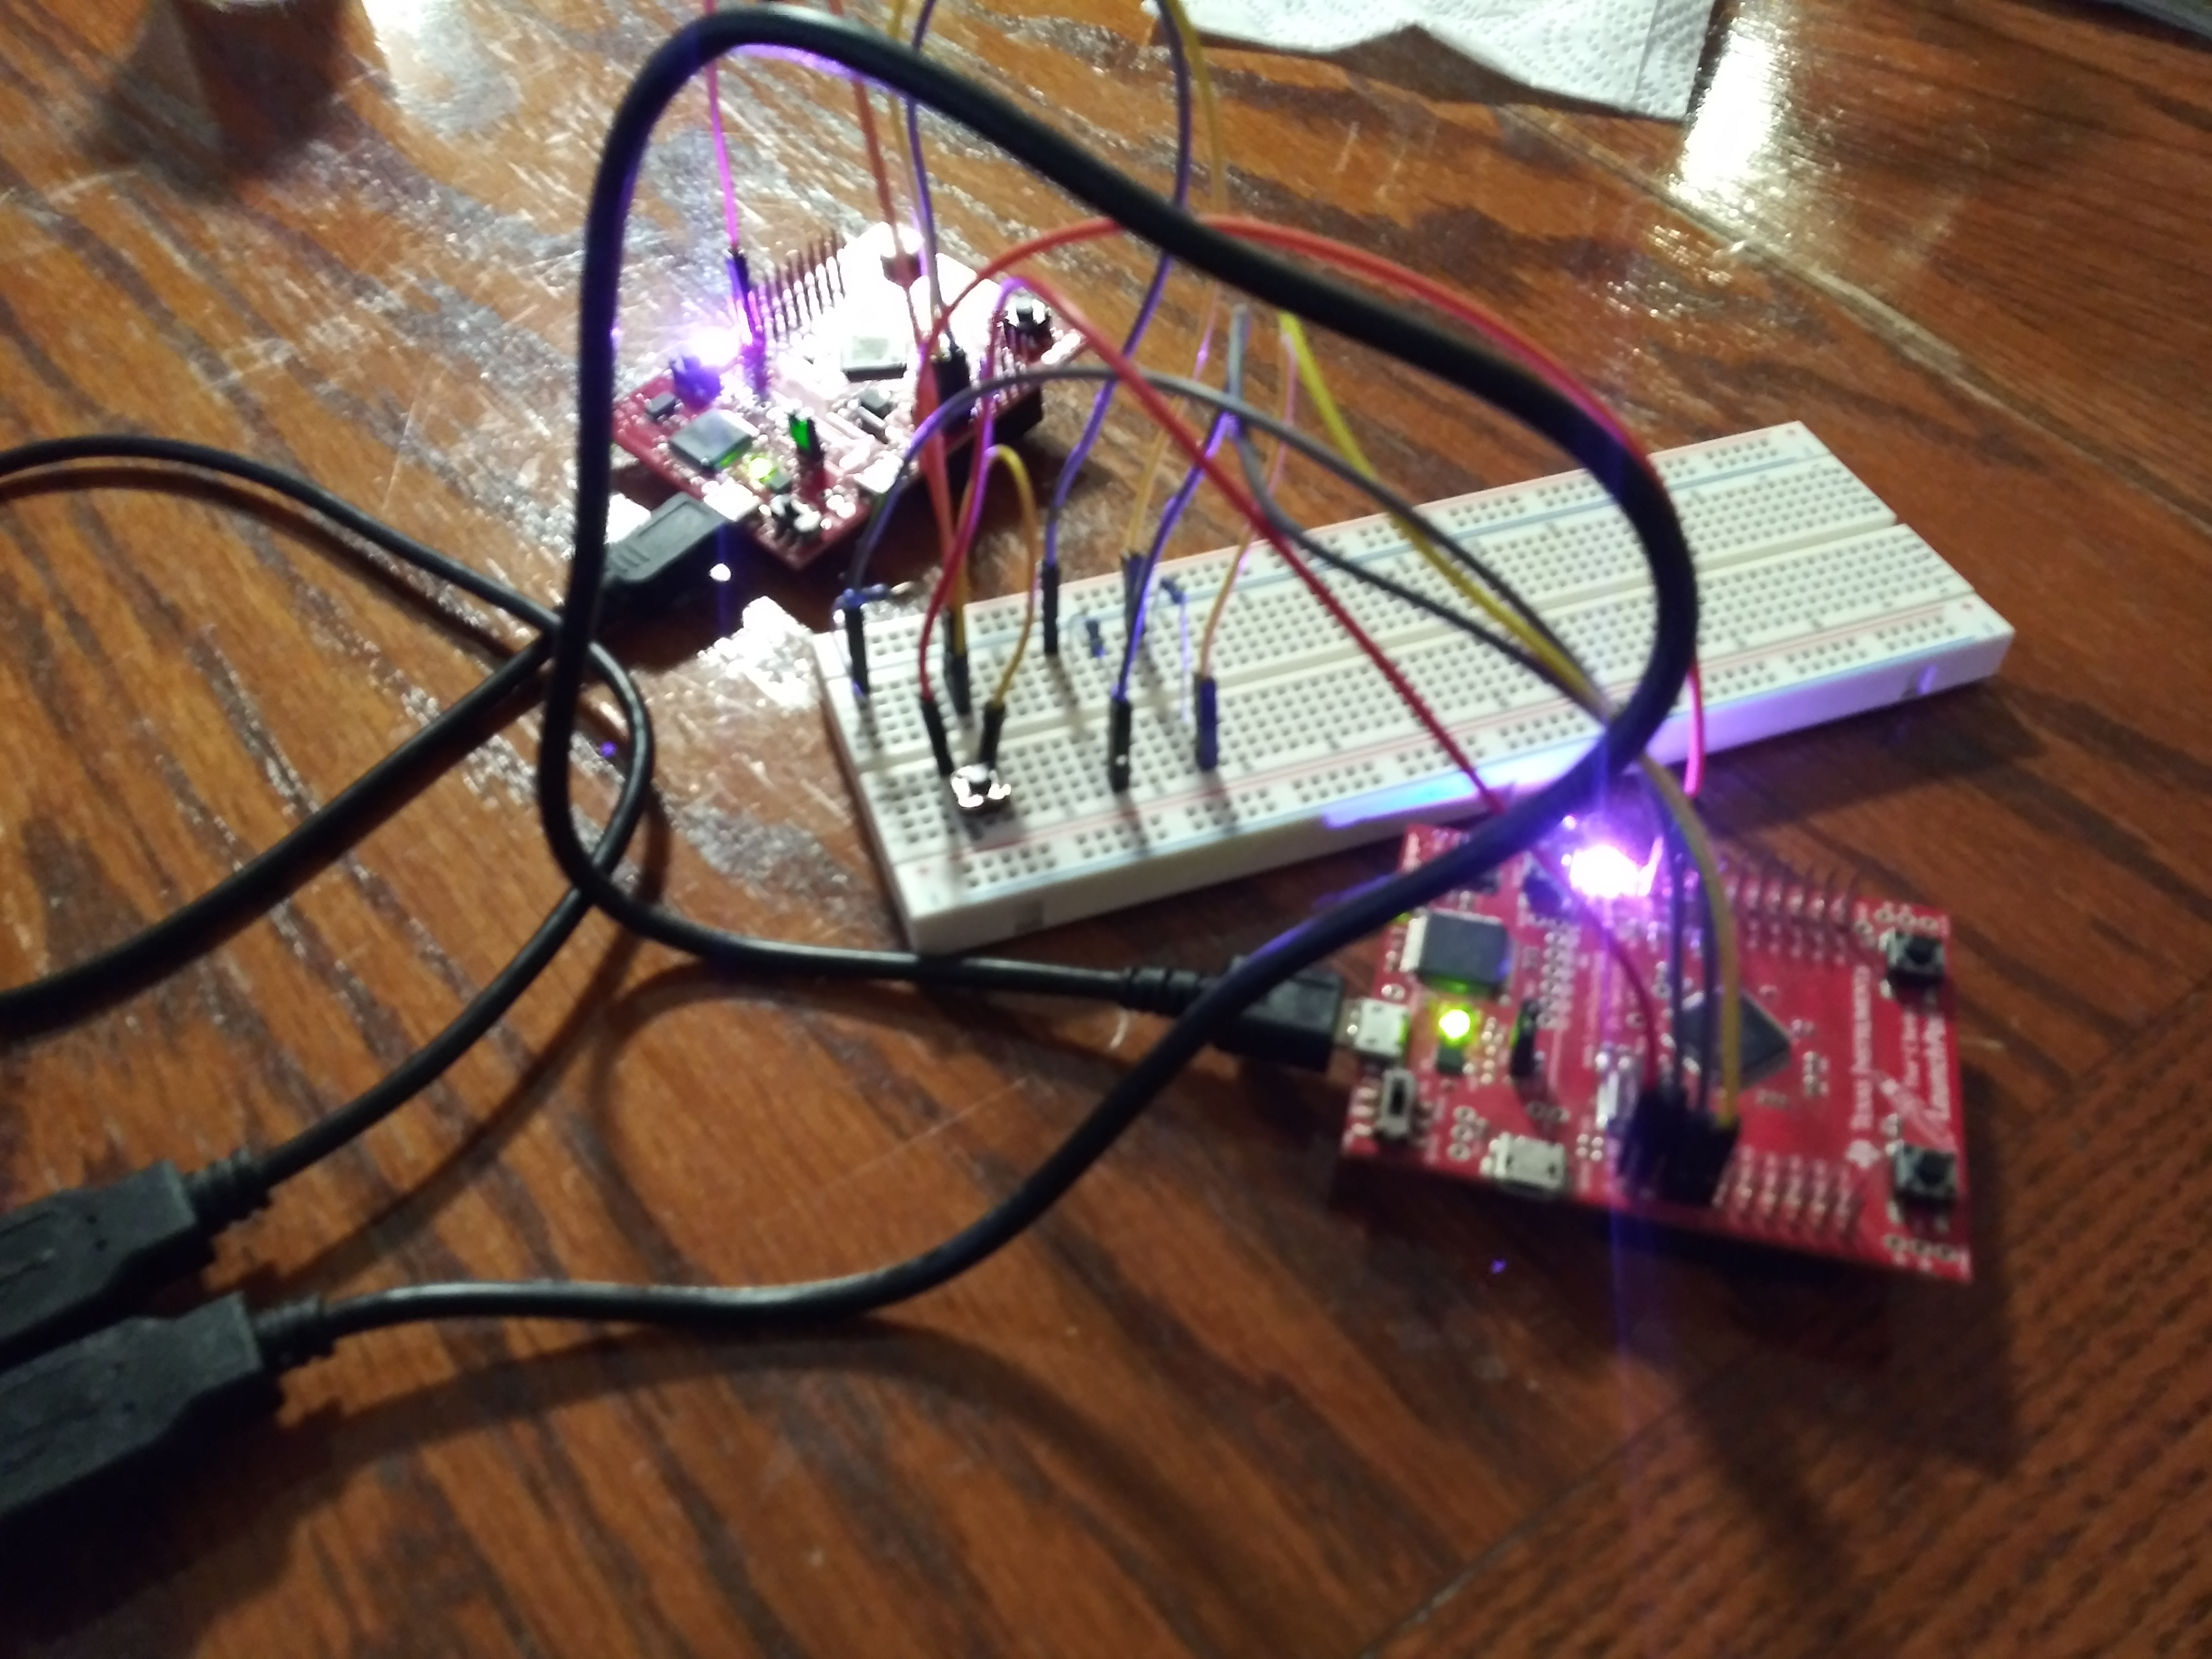
\includegraphics[width=\textwidth]{Images/20211013_213328}
	\caption{Picture of embedded system on Mode 2.}
	\label{picture}
\end{figure}

\section{Software Design}
In order to properly be able to switch modes at any given time,
I have all three modes in functions. If the interrupt is
detected, it raises a flag, and the flag quits out of the
current function (mode) and goes to the menu.

\section{Conclusion}
Implementing Modes 1 and 2 was very simple and easy (it took
less than one hour to set everything up for each mode).
Implementing Mode 3 and the interrupt took an incredibly
disproportionate amount of time in comparison.
If I had not come up with
the handshake protocol, I would not have finished the project.
I learned the importance of verifying information to be sent,
and can only think of the TCP/IP protocols that we use on a
day-to-day basis. A lot of work was put into making sure
data is transmitted quickly and reliably across the Internet,
and I only scratched the surface of what is required today.

\end{document}
